%We will now discuss  an example demonstrating the need to describe attenuation in specifications.
\emph{Attenuation} is the ability to give restricted access to an object's functionality. Thus is usually done thorugh
introduction of an intermediate object. While it is a common programming practice the term was coined, and the practice 
was studied in detail in the object capabilities literature \cite{millerPhD}. 

The example of attenuating the DOM was proposed in \cite{dd}. 
In this section we revisit that example, and use it to motivate the need for holistic specifications, to give an informal introduction
to  our language for such holistic specifications. We also argue that compared with the soecifcation in \cite{dd}, our specification xxxx.

This example deals with a tree of DOM nodes: Access to a DOM node gives access to all its parent and children nodes, and the ability to modify the node's properties. However, as the top nodes of the tree usually contain privileged information, while the lower nodes contain less crucial information, such as xxxx, we want to be able to limit  the access that we give  to third parties to only part of the DOM tree. We do this through \prg{Wrapper}, which has a field \prg{node} pointing to a \prg{Node}, and a field \prg{height} which restricts the range of \prg{Node}s which may be modified through the use of the particular \prg{Wrapper}. Namely, when you hold a \prg{Wrapper}  you can modify the \prg{property} of all the descendants    and also all the \prg{height}-th ancestors of the \prg{node} of that particular \prg{Wtrapper}.

The corresponding code appears in Figure \ref{fig:DOM}. 
We write our code in a small fictitious class-based, dynamically typed, imperative programming language. All functions are public, \ie may be called by any other object, and all fields are private, \ie may be read or written only by the object itself. 

\begin{figure}[htb]
\begin{tabular}{llll}
&
\begin{minipage}{0.40\textwidth}
\begin{lstlisting}
class Node(par,prop){

  fld parent = par;
  fld property = prop;
  fld children = new array[10];
  fld maxChild=0;
  children[maxChild++]=this
  
  func getParent(){
       parent 
  }  
  func getChild(i){
       children[i] 
  }
  func setProperty(prp){
       property = prp 
  }  
  func setChild(nd){
       children[i] = nd
  }  
}
\end{lstlisting}
\end{minipage}
& & 
\begin{minipage}{0.40\textwidth}
\begin{lstlisting}
class Wrapper(nd,hgt){

  fld node=nd;
  fld height=hgt;

  func setPropety(i,prp){
    if (i>height){ 
       return 
    } 
    else  
    {  nd=node;  
       while (i>0){
          nd=nd.getParent();
          i--;    };
        nd.setProperty(prp); }
  }    
  func getChild(i){ 
    Wrapper(node.getChild(i),
                    height+1); 
 }                           
}
\end{lstlisting}
\end{minipage}
\end{tabular}
 \vspace*{-7mm}
\caption{DOM - \prg{Node}  and \prg{Wrapper} }
\label{fig:DOM}
\end{figure}

In Figure we show an example of the use of  \prg{Wrapper} objects to attenuate the use of \prg{Node}s\footnote{SD: Is that a good sentence?}  The function \prg{usingWrappers} takes as parameter an object of unknown provenance, here called \prg{unknwn}. On lines 2-7 it creates a tree, consisting of nodes \prg{n1}, \prg{n2}, ... \prg{n6}, depicted as blue circles on the   right-hand-side of the Figure. On line 8 it creates a wrapper of \prg{n5} with height \prg{1}. This means that the wrapper \prg{w} may be used to modify \prg{n3}, \prg{n5} and \prg{n6} (\ie the objects in the green triangle), while it cannot be used to modify \prg{n1}, \prg{n2}, and \prg{4} (\ie the objects within the blue triangle). 

On line 8 we call the function \prg{untrusted} on the \prg{unknown} object, and pass \prg{w} as an argument. This means that \prg{unknown} obtains access to \prg{w}, which in turn has transitively access to all  \prg{Node}-s in the tree. Nevertheless, we know that the call to the \prg{untrusted} function is guaranteed no to affect the values of the \prg{property} field of the nodes \prg{n1}, \prg{n2}, and \prg{4}. Thus, the assertion on line 10 is guaranteed to succeed.

\begin{figure}[htb]
\begin{tabular}{llll}
&
\begin{minipage}{0.50\textwidth}
\begin{lstlisting}
func usingWrappers(unknwn){
   n1=Node(null,"fixed"); 
   n2=Node(n1,"robust"); 
   n3=Node(n2,"volatile"); 
   n4=Node(n2,"const");
   n5=Node(n3,"variable");
   n6=Node(n3,"ethereal");
   w=Wrapper(n5,1);
   unknwn.untrusted(w);
   assert  n2.property == "robust" 
   ...
}
\end{lstlisting}
\end{minipage}
& & 
\begin{minipage}{0.75\textwidth}
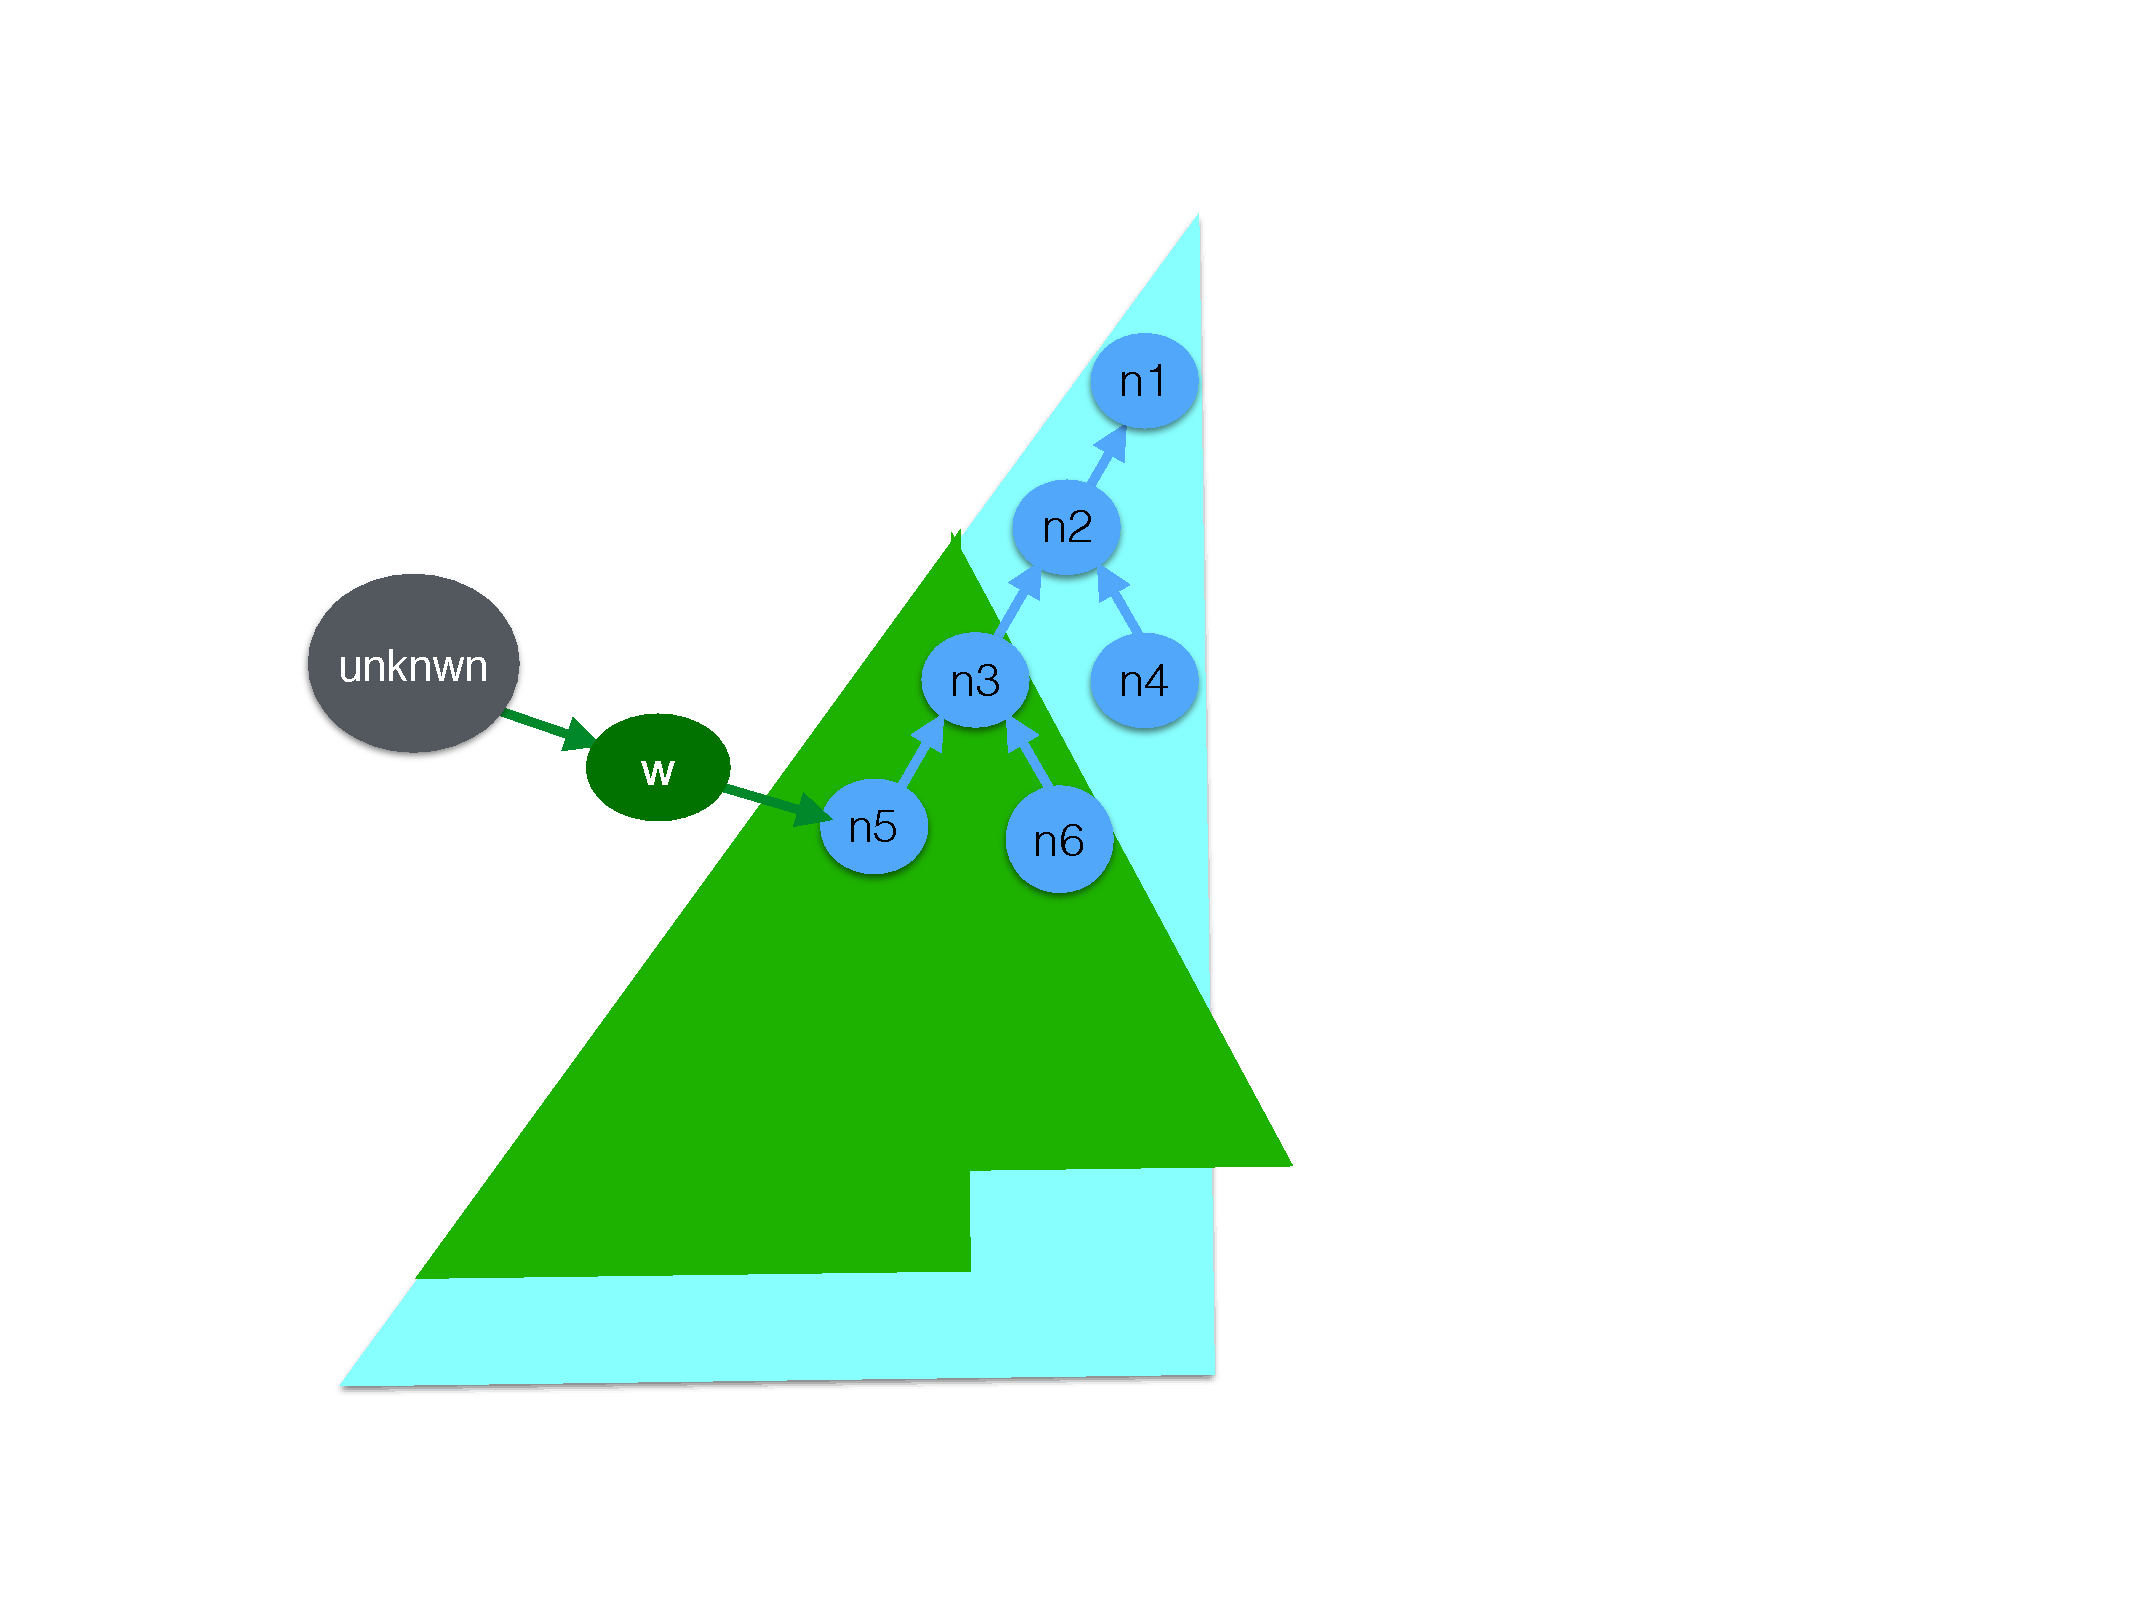
\includegraphics[width=\linewidth, trim=145  320 60 105,clip]{diagrams/DOM.pdf}
% x y z w
% y seems to eat up the bollom
% y=320 is good
% x eats space from left, if you increase it the diagram decreases from left
% w eats space from top, if you increase it the diagram decreases from top
% w=100 is good
%\includegraphics[page=3, width=\linewidth, trim=150  270 40 150, clip]{diagrams/snmalloc.pdf}\sdcomment{I think we need to change the diagram so that it says small slab.}
\end{minipage}
\end{tabular}
 \vspace*{-1mm}
\caption{\prg{Wrapper}s protecting \prg{Node}s }
\label{fig:WrapperUse}
\end{figure}
 